
\subsection{The Crank--Nicolson Method}
\begin{frame}{The Crank-Nicolson Method}

\begin{block}{}
   \center{symmetry in the construction of difference equations \\ $\rightarrow$
better accurancy} 
 \end{block}
 
\begin{equation}\underline{\frac{\partial u}{\partial t} \Big \vert _{A}\cong \frac{u(x,t) - u(x,t - h)}{k}}\end{equation} w oparciu o punkty symetryczne wzgl. A
 
 \centerline{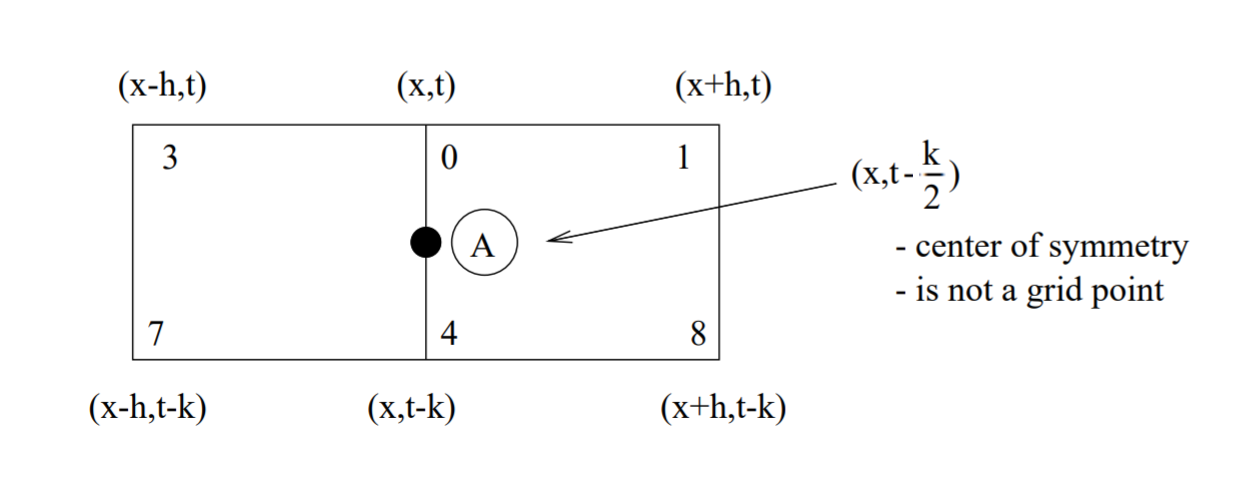
\includegraphics[width = 1 \linewidth]{img/23/crank}}
\end{frame}

\begin{frame}
\begin{equation} \frac{\partial ^2 u}{\partial x^2} \Big \vert _{4}\approx \frac{u(x - h,t - k) - 2 \cdot u(x,t - k) + u(x + h, t - k)}{h^2}\end{equation}
\begin{equation} \frac{\partial ^2 u}{\partial x^2} \Big \vert _{0}\approx \frac{u(x - h,t) - 2 \cdot u(x,t) + u(x + h, t)}{h^2} \end{equation}
to:
\begin{equation} \frac{\partial ^2 u}{\partial x^2} \big \vert _{A} = \frac{1}{2} \cdot \left ( \frac{\partial ^2 u}{\partial x^2} \Big \vert _{0} + \frac{\partial ^2 u}{\partial x^2} \Big \vert _{4} \right )\end{equation}
\textbf{W met. ,,Implicit'' wprowadzamy:}
\begin{multline} \lambda \cdot u(x-h,t) - (1+2 \cdot \lambda)\cdot u(x,t) + \lambda \cdot (x+h,t) = \\
 -\lambda \cdot u(x-h,t-k) - (1-2 \cdot \lambda) \cdot u(x,t-k) - \lambda \cdot u(x+h,t-k)\end{multline}
czyli:
$$ \underline{\lambda \cdot u_3 - (1+2 \cdot \lambda) u_0 + \lambda u_1 = -\lambda \cdot u_7 - (1-2 \cdot \lambda) u_4 - \lambda u_8}$$
\end{frame}